\documentclass{beamer}
\usepackage[english]{babel}
\usepackage[utf8]{inputenc}
\mode<presentation>{\usetheme{FS18}}
\usepackage{amsmath,amsthm, amssymb, latexsym}
\usepackage[orientation=portrait,size=a0,scale=1.4]{beamerposter}
\usepackage{natbib}
\graphicspath{{../figures/graphics/}}
 
\title{Applying a Reduced Model of Apical and Basal Dendritic Compartments to Sequence Learning in Recurrent Neural Networks}
\author{Fabian Schubert, Claudius Gros}
\institute{Institute for Theoretical Physics, Goethe University Frankfurt a.M.}
%\date[Feb. 28th, 2018]{Feb. 28th, 2018}


\begin{document}
\begin{frame}[t]
\begin{columns}[t]
\begin{column}{.4\textwidth}

\begin{myblock}{Introduction}
\begin{itemize}
\item Experiments suggest that, depending on the amount of apical (distal) and basal dendritic synaptic drive, layer 5 pyramidal neurons can exhibit quietness, low frequency spiking and high frequency bursting \cite{Letzkus_2006,Shai_2015}.
\item The latter only occurs when distal and basal inputs coincide in time. A simplified, rate based compartment model of this effect has been used to gate plasticity of basal connections by means of distal synaptic inputs \cite{Bono_2017}.
\item We use this mechanism for sequence prediction. In our framework, coincidence detection of distal and basal input modulates plasticity to extract a predictive signal from a recurrent dynamic reservoir.
\item This approach is similar to echo state networks \cite{Jaeger_2010}, but readout and external input are now collected by the same units (see Fig.~\ref{fig:Model_Illustration}). Combining both streams of information in the previously described manner, the error signal for learning is thus implicitly expressed as the nonlinear response to basal and distal input.
\end{itemize}
\end{myblock}

\begin{myblock}{Model Description}
We used a discrete time non-binary rate encoding neuron model, whose output frequency is given by
\begin{align*}
x\left(I_p,I_d\right) &= 2 \left[ \sigma\left(I_p-\theta_{p1}\right) \sigma\left(I_d-\theta_d\right)\ +\alpha\sigma\left(I_p-\theta_{p0}\right)\sigma\left(-\left(I_d-\theta_d\right)\right)\right] - 1 \\
\sigma\left(x\right) &= \frac{1}{1+\exp(-g\cdot x)} \\
I_p (t) &= \sum_{k=1}^n w_{p,k} (t) x_{p,k} (t) , \;\;\; I_d (t) = \sum_{k=1}^n w_{d,k} (t) x_{d,k} (t)
\end{align*}
Proximal and distal weights were subject to Hebbian plasticity and weight normalization.
\begin{align*}
\Delta w_{p/d,i} (t) &= \epsilon_w \left(x(t)-\langle x \rangle\right)\left(x_{p/d,i}(t)-\langle x_{p/d,i} \rangle \right) \\
w_{p/d,i}(t+1) &= w_{p/d,\rm total} \frac{w_{p/d,i}(t) + \Delta w_{p/d,i}(t)}{\sqrt{\sum_{k=1}^{np/nd} \left[ w_{pk}(t) + \Delta w_{pk}(t) \right]^2}}
\end{align*}
\end{myblock}

\begin{myblock}{A Single Distal Input Stream Acts as a Guiding Signal for Proximal Plasticity}
\begin{itemize}
\item We fed a single neuron with 10 randomly fluctuating proximal inputs and one distal input that was perfectly correlated with one of the proximal signals. 
\item As a ``distraction", the standard deviation of another proximal input was increased, such that proximal inputs had a dominant principal component.
\item As shown in Fig.~\ref{fig:Results_1}, the distal input acts as a guiding input, such that the proximal input that maximizes correlation with the distal input is selected.
\item If the distal input is uncorrelated, proximal weights select the principal component (Fig.~\ref{fig:Results_2}).
\end{itemize}
\end{myblock}

\begin{myblock}{Conclusions}
\begin{itemize}
\item The model allows for the reproduction of a wide range of dynamical properties of spiking neurons.
\item Characteristic properties such as the spike height and width can be controlled very well by certain model parameters.
\item Good usability as a rate encoding model with a sigmoid activation function.
\item Further investigations should compare how spiking and rate network dynamics map onto each other under the same synaptic coupling.
\end{itemize}
\end{myblock}

\end{column}

\begin{column}{.5\textwidth}
\begin{figure}
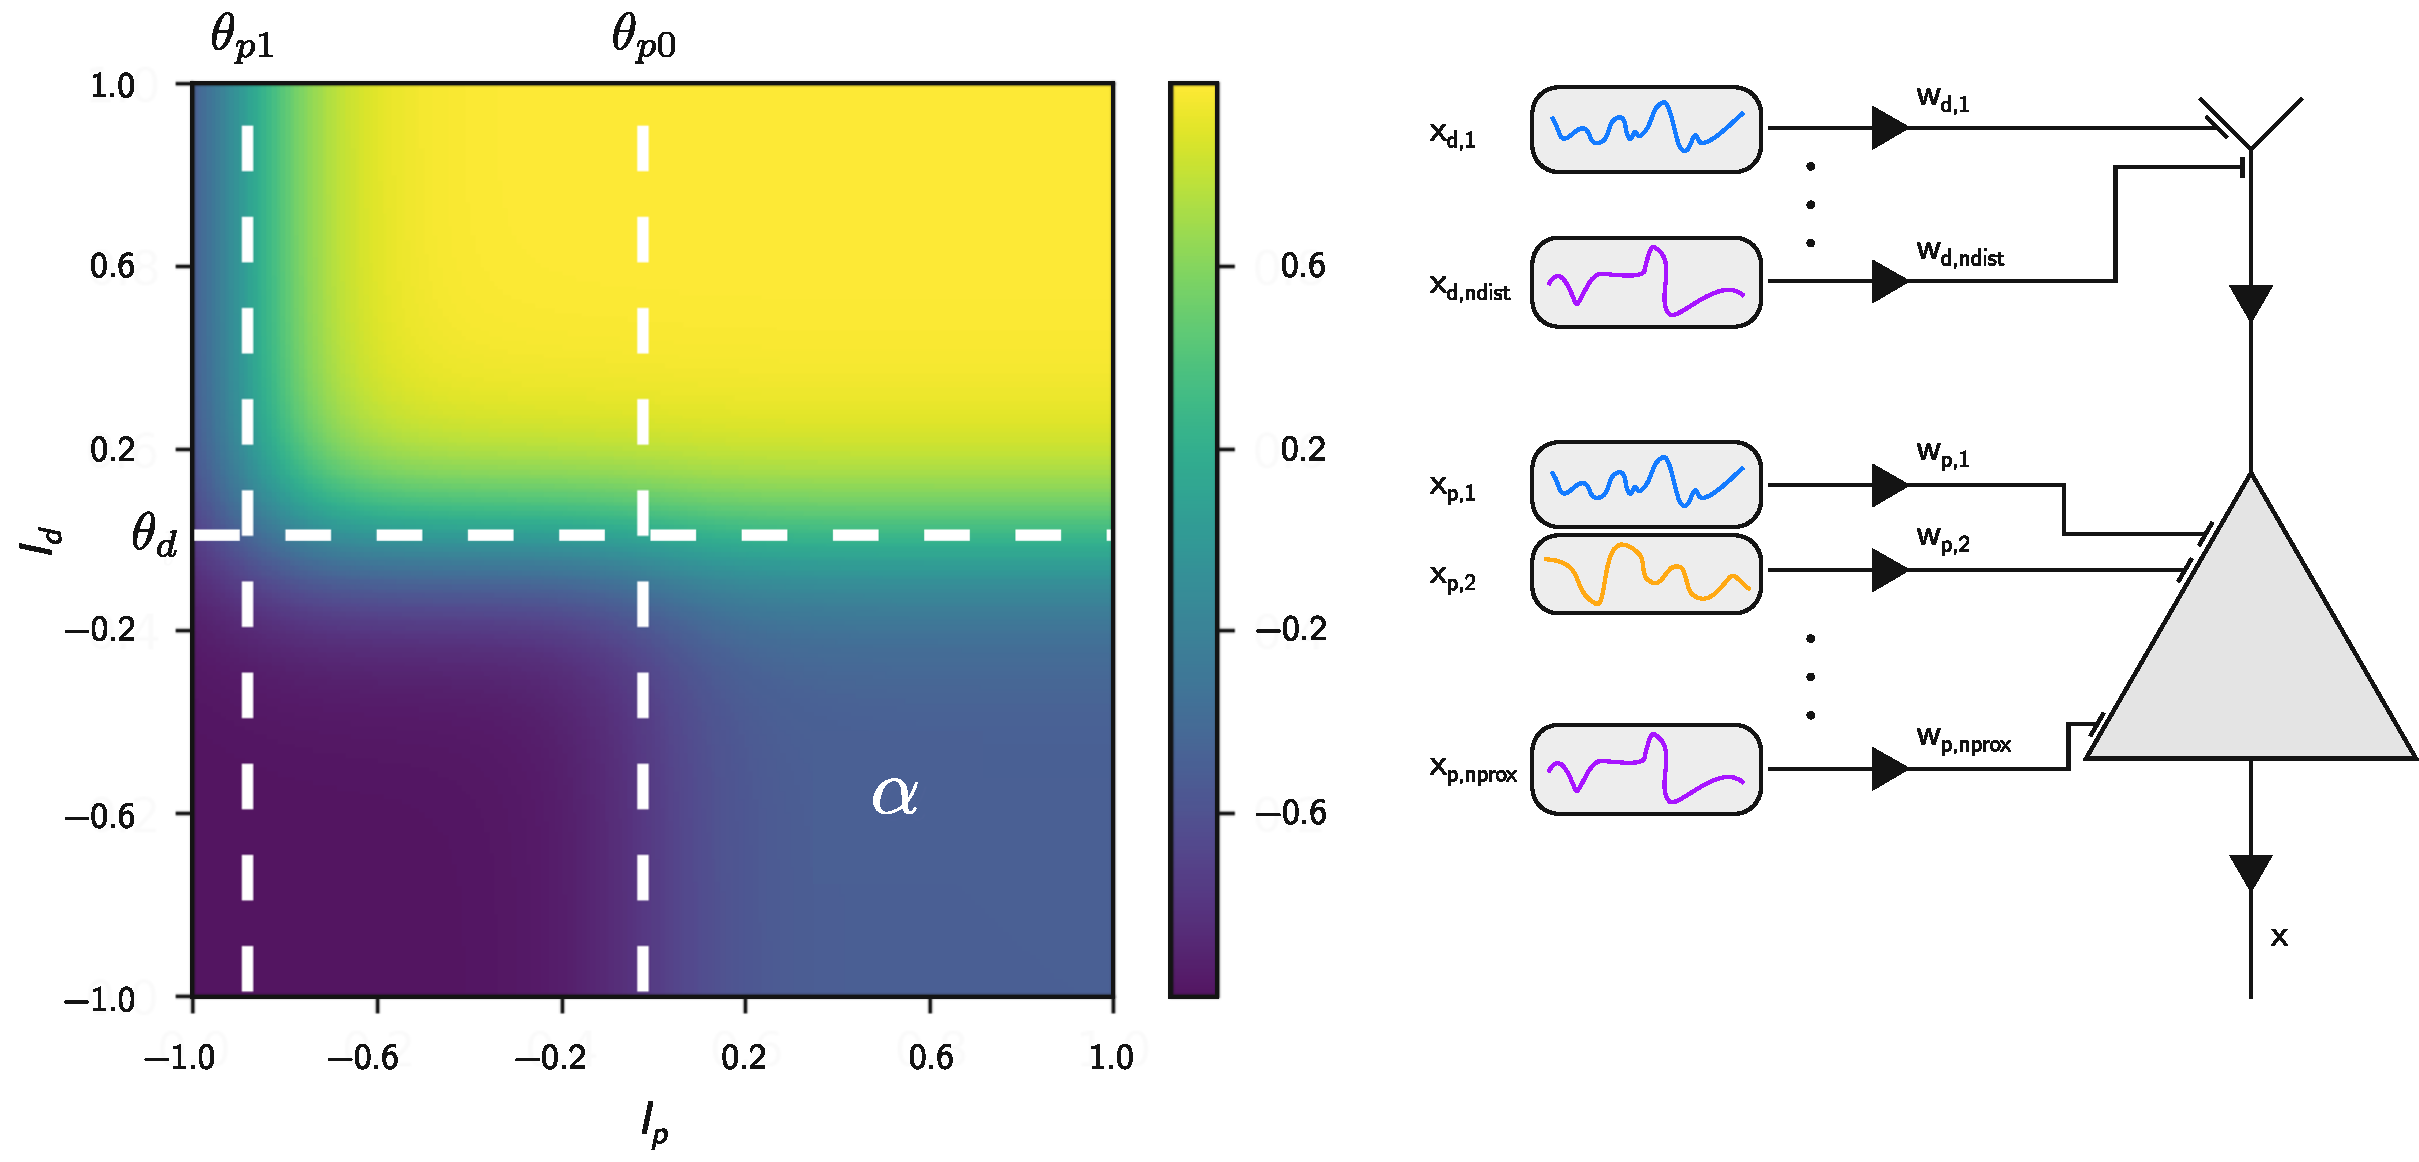
\includegraphics[width=\textwidth]{../figures/fig1.pdf}
\caption{Output rate model a function of proximal (basal) and distal (apical) dendritic input (left) and an illustration of the accumulation of inputs in the neuron model.}
\label{fig:Model_Illustration}
\end{figure}

\begin{figure}
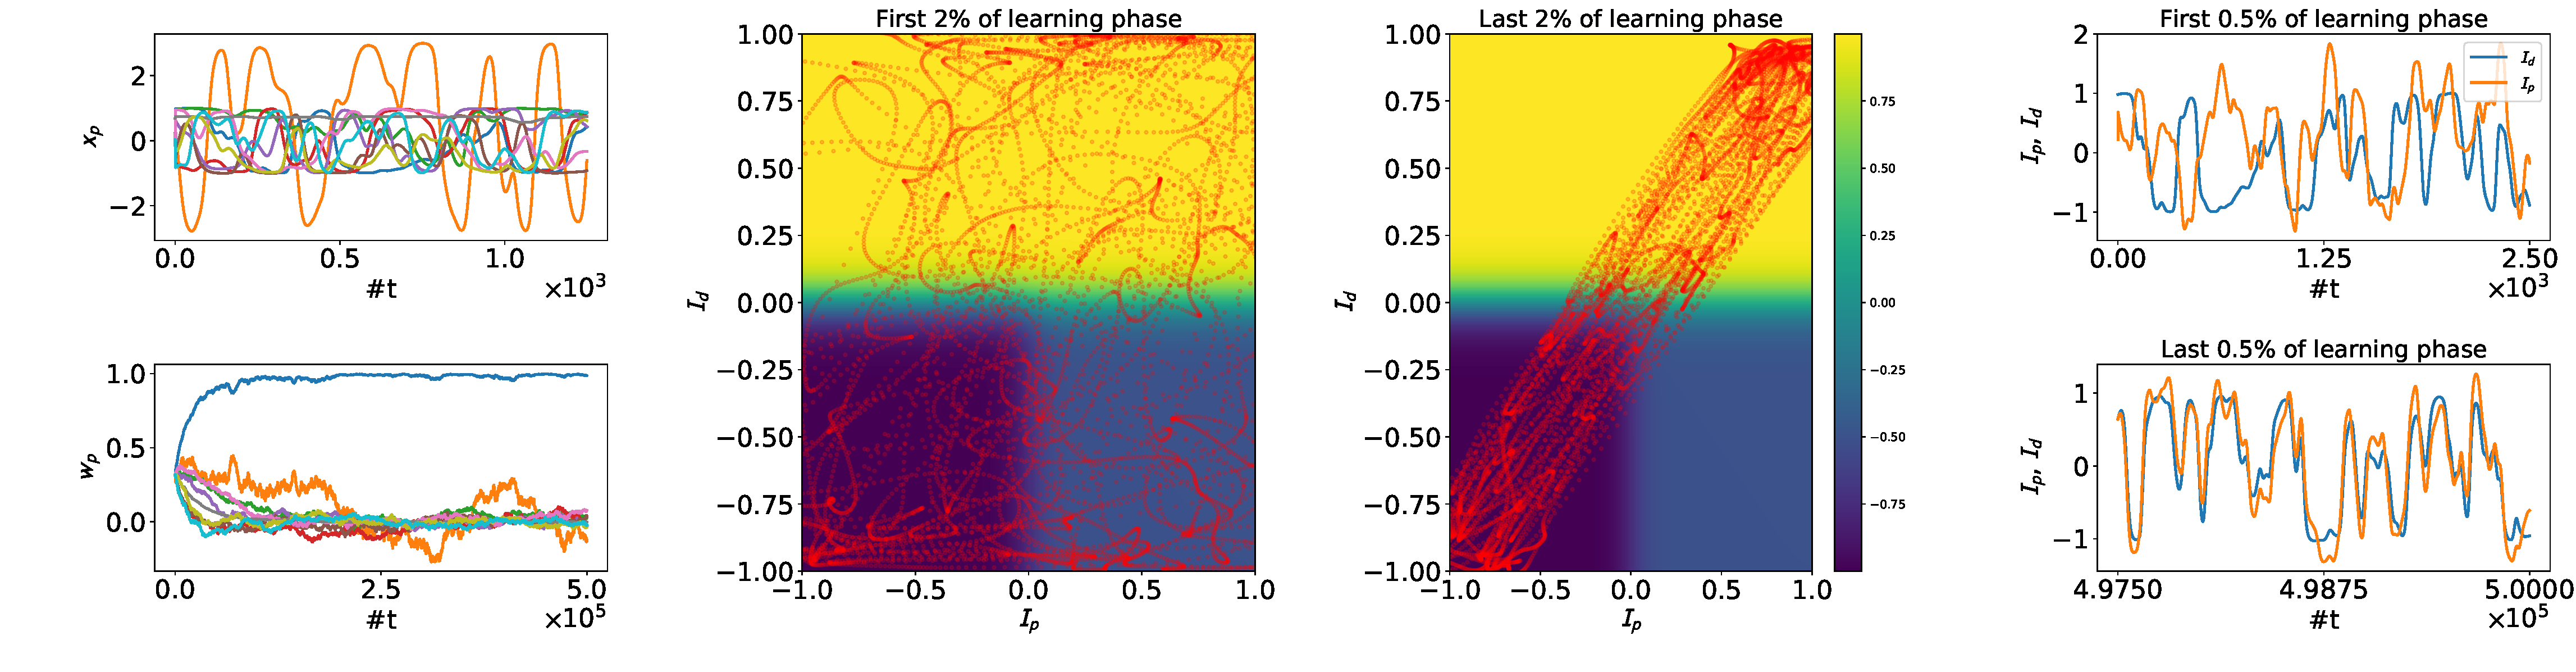
\includegraphics[width=\textwidth]{../figures/fig2.pdf}
\caption{Results for a single distal input, correlated with one proximal input}
\label{fig:Results_1}
\end{figure}

\begin{figure}
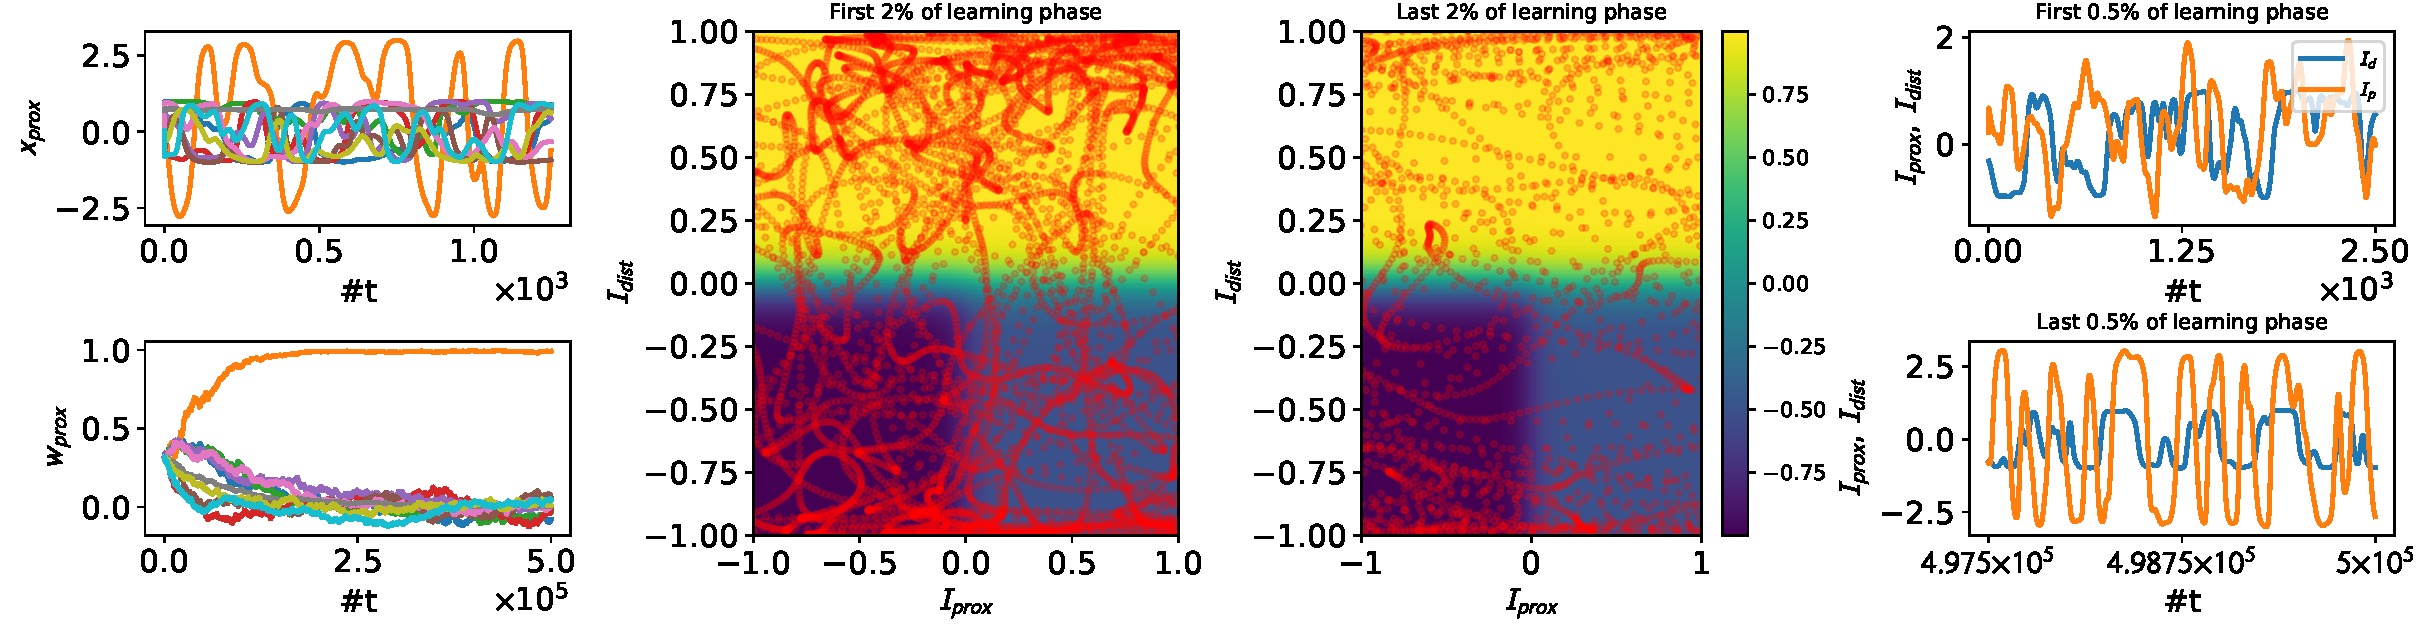
\includegraphics[width=\textwidth]{../figures/fig3.pdf}
\caption{Single distal input, uncorrelated}
\label{fig:Results_2}
\end{figure}

\begin{figure}
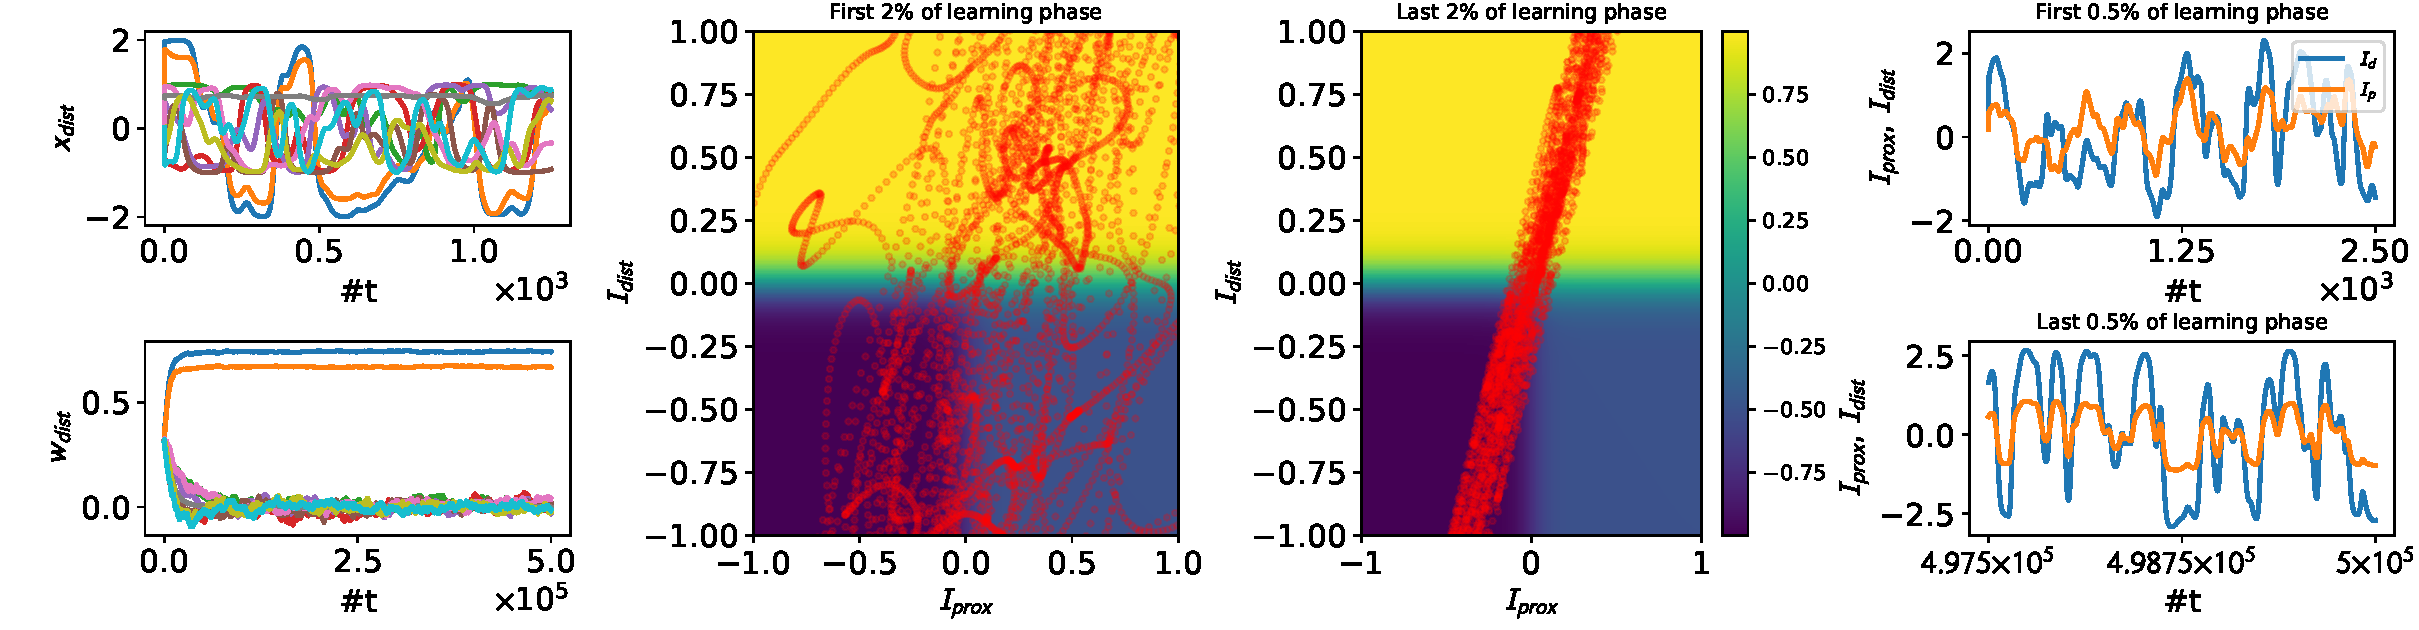
\includegraphics[width=\textwidth]{../figures/fig4.pdf}
\caption{Echo state network}
\label{fig:Results_3}
\end{figure}

\noindent\rule{\textwidth}{2px}
\begin{small}
\bibliographystyle{unsrt}
\bibliography{poster_citations}
\end{small}
\end{column}
\end{columns}
\end{frame}
\end{document}
